\section{Architecture}
\label{sec:architecture}

This chapter describes the architecture of Stress+.
The whole architecture was designed in a way that arbitrary stress tests with different modules can be created very easily.
It was also considered that programming and adding new modules is very simple.
Each stress test consists of a pipeline of screens which are shown to the participant successively in the specified order.
Additionally, a stress test can contain overlays which are displayed on top of the screens.

\begin{figure}[htb]
  \centering
  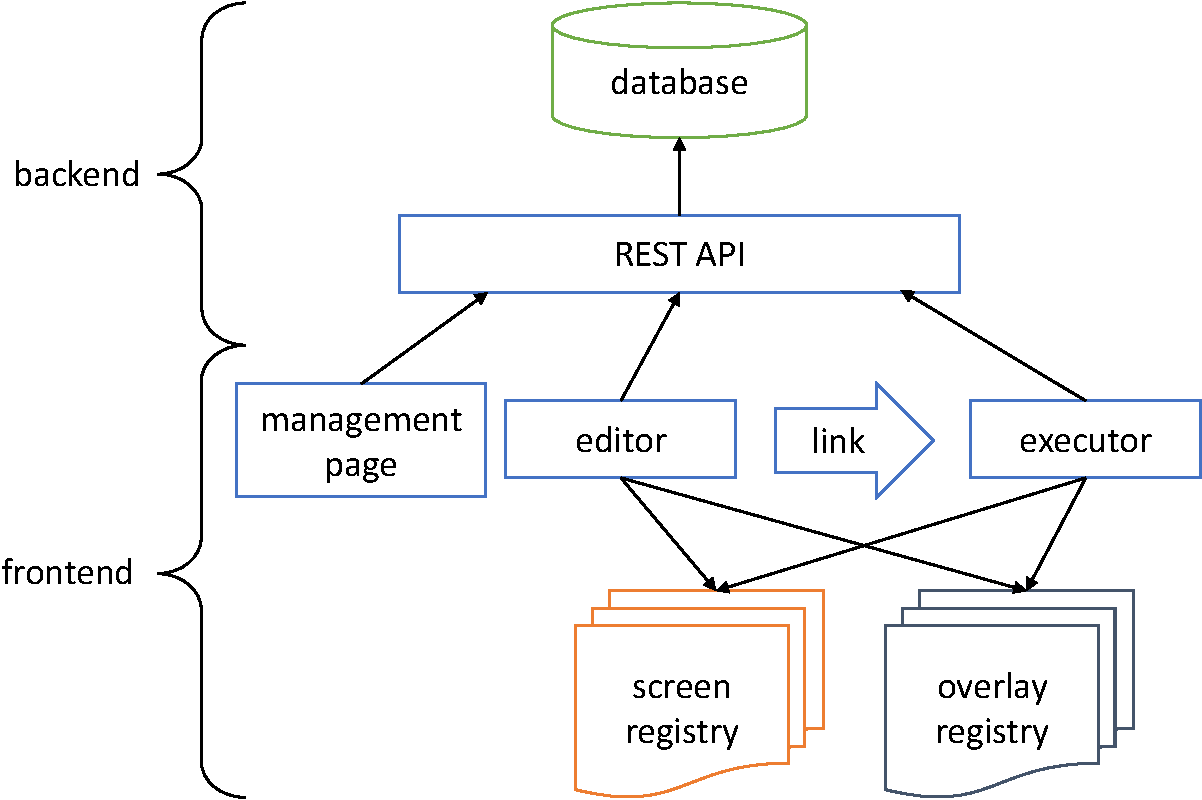
\includegraphics[width=\textwidth]{figures/Architecture-crop}
  \caption{Software architecture}
  \label{fig:software-architecture}
\end{figure}

The figure \ref{fig:software-architecture} shows the software architecture of Stress+.
It is a browser-based \mbox{application} and consists of a frontend and a backend.
The main frontend components of Stress+ are the editor for creating and editing stress tests and the executor for executing the stress test.
The third frontend component is the management page, on which all available stress tests can be managed.
To be able to easily add new modules in the future all available screens and overlays are registered in the screen registry and overlay registry. 
Therefore, the editor and executor are developed generically without the knowledge of the available modules.
They must query the registries to know which modules are currently present.
After saving a stress test in the editor a link is generated, which can be sent to the participant so he can execute the stress test.

The backend is responsible for saving the stress test configurations and the statistics on how the participant performed.
Therefore, it consists of a REST API, through which the database can be accessed.

\subsection{Frontend}
The frontend is a single-page application written in JavaScript utilizing the React framework. 
The following sections describe the different frontend components in more detail.

\subsubsection*{Screen}
The stress test consists of a list of screens that will be displayed successively to the participant. 
A screen will be displayed full screen inside the user's browser. 
Each screen has its own settings, which can be adjusted inside the editor. 
All available screens are listed in chapter \ref{sec:screens}.

\subsubsection*{Overlay}
The stress test can be equipped with overlays that are displayed on top of the current screen. 
Because all overlays are displayed simultaneously during the whole stress pipeline execution, they do not have an order. 
Each overlay has its own settings, which can be adjusted inside the editor.
All available overlays are listed in chapter \ref{sec:overlays}.

\subsubsection*{Management page}
On the management page, all available stress tests are displayed.
From there you can open a stress test in the editor, delete one or create a new test.
Further details about the management page can be found in chapter \ref{sec:management-page}.

\subsubsection*{Editor}
The stress tests can be created and edited in the editor.
Also, every setting of the screens and overlays can be adjusted within the editor.
Each stress test has a unique id that is generated when it is saved for the first time.
With this id a link is generated that can be used by the participants to execute the stress test.
From the editor, users can also download all recorded statistics for the current stress test.
Chapter \ref{sec:editor} presents further details about the editor.

\subsubsection*{Executor}
The executor is responsible for executing the stress test specified by the link.
It will display each screen successively to the participant and show all overlays simultaneously during the whole stress test execution.
The executor also collects records from the screens and persist them in the database.
Further details can be found in chapter \ref{sec:executor}.

\subsection{Backend}
The backend consists of the database and the REST API

\subsubsection*{Database}
To save the stress test configurations and the results of stress test executions a database is used.
The data does not have a fixed structure, as arbitrary modules can be composed together in a stress test.
Therefore, the document-oriented NoSQL database MongoDB is used instead of a relational database.

\subsubsection*{REST API}
The REST API acts as the connection between the frontend and the database.
It can be accessed via HTTP and uses JSON documents for transferring the data.
The REST API endpoints are written in JavaScript on the NodeJS platform.
